\documentclass[tikz,border=4pt]{standalone}
\usepackage{amsmath,amssymb}
\usepackage{xcolor}
\usetikzlibrary{arrows.meta,matrix,calc}
\definecolor{forestgreen}{rgb}{0.0,0.5,0.0}
\definecolor{lightblue}{rgb}{0.4,0.75,1.0}

\begin{document}
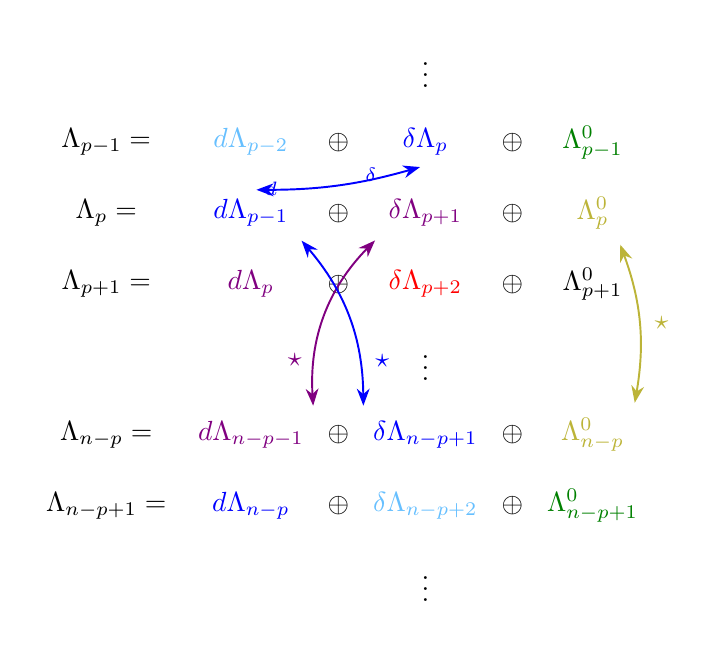
\begin{tikzpicture}[
  >=Stealth,
  every node/.style={font=\normalsize},
  map/.style={<->,line width=0.7pt,shorten >=2pt,shorten <=2pt}
]
  \matrix (m) [matrix of math nodes,column sep=2pt,row sep=7pt,nodes={anchor=center}] {
    & & & \vdots & & \\
    \Lambda_{p-1}={}& {\color{lightblue}d\Lambda_{p-2}} & \oplus & |[name=delp]|{\color{blue}\delta\Lambda_p} & \oplus & {\color{forestgreen}\Lambda_{p-1}^{0}} \\
    \Lambda_p={}& |[name=dp]|{\color{blue}d\Lambda_{p-1}} & \oplus & |[name=delp1]|{\color{violet}\delta\Lambda_{p+1}} & \oplus & |[name=hp]|{\color{yellow!70!black}\Lambda_p^{0}} \\
    \Lambda_{p+1}={}& {\color{violet}d\Lambda_p} & \oplus & {\color{red}\delta\Lambda_{p+2}} & \oplus & \Lambda_{p+1}^{0} \\
    & & & \vdots & & \\
    \Lambda_{n-p}={}& |[name=dnp]|{\color{violet}d\Lambda_{n-p-1}} & \oplus & |[name=delnp]|{\color{blue}\delta\Lambda_{n-p+1}} & \oplus & |[name=hnp]|{\color{yellow!70!black}\Lambda_{n-p}^{0}} \\
    \Lambda_{n-p+1}={}& {\color{blue}d\Lambda_{n-p}} & \oplus & {\color{lightblue}\delta\Lambda_{n-p+2}} & \oplus & {\color{forestgreen}\Lambda_{n-p+1}^{0}} \\
    & & & \vdots & & \\
  };

  \draw[map,blue] (delp.south) to[bend left=8]
    node[pos=0.18,left=2pt,font=\scriptsize] {$\delta$}
    node[pos=0.78,left=2pt,font=\scriptsize] {$d$} (dp.north);
  \draw[map,yellow!70!black] (hp.south east) to[bend left=15]
    node[right=2pt] {$\star$} (hnp.north east);
  \draw[map,violet] (delp1.south west) to[bend right=24]
    node[near end,left=1pt] {$\star$} (dnp.north east);
  \draw[map,blue] (dp.south east) to[bend left=20]
    node[near end,right=2pt] {$\star$} (delnp.north west);
\end{tikzpicture}
\end{document}
